\section{Problem Formulation}
\label{sec:problem}

The grasp planning problem is composed of four sub-problems: state estimation, grasp synthesis, grasp planning and control. A typical approach is to represent the belief state using prior distributions (often a Gaussian), select a grasp robust in the face of uncertainty (be it pose uncertainty or shape incompleteness) and  finally to use tactile feedback to adjust the grasping trajectory, see e.g.~\citep{bib:nikandrova_2014}. The reach-to-grasp trajectory is typically computed using some conventional sampling-based techniques which minimise the cost, in Euclidean space, of moving the robot's end effector to the selected grasp configuration. Comparatively little work has explored the more complex problem of reasoning about uncertainty while planning this dexterous reach-to-grasp trajectory. This is mainly due to the high dimensionality of the configuration space of a dexterous manipulator.  In this work we consider precisely this problem. First we formulate the problem of reducing uncertainty in object pose, and then show how to formulate a reach to grasp problem that incorporates this measure.

\begin{figure}[t]
\centerline{
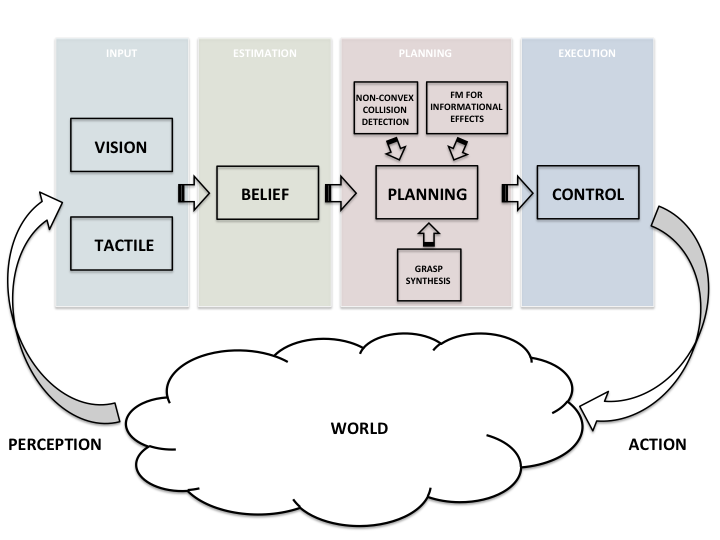
\includegraphics[width=.98\columnwidth]{img/ch07_architecture.png}
}
\caption[SPAM-PLAN for grasping]{The system architecture comprises sensory input, pose estimation, motion planning and active control.}
\label{fig:architecture}
\end{figure}

\subsection{Problem formulation}
%
%- mainly in real-world problem inferring the pose of an object produces a non-Gaussian pdf
%- introduction of (with some maths)
%-- transition function
%-- observation function
%-- objective function we want to minimise

This section is concerned with the problem of planning control actions to reach a goal state in the presence of incomplete or noisy observations. Let us consider a discrete-time system with continuous non-linear deterministic dynamics, 
$$
x_{t+1}=f(x_t,u_t) 
$$ 
where $x_{t}\in\mathbb{R}^n$ is a configuration state of the robot and $u_{t}\in\mathbb{R}^l$ is a action vector, both parametrised over time $t\in\{1,2,...\}$.
Let $p\in SE(3)$ describe the object pose, given an initial prior belief state $b_1$ and let us define a set of $k$ hypotheses as $\{p^i\}_{i=1}^k$, where $p^1=\arg\max b_1$ and $p^i\sim b_1,i\in[2,k]$. 

We know that in general the problem of planning in belief space is intractable. Instead let us consider a method to search for a sequence of actions, $u_{1:T-1}=\{u_1,\dots,u_{T-1}\}$, that distinguish between observations that would occur if the object were in some pose $p^1$, from those that would occur in some other poses $p^i$, with $i\in[2,k]$.
At each time step, $t$, the system will make an observation, $y\in\mathbb{R}^m$, that is a non-linear stochastic function of the joint state of the robot and some object state. 
%$$
%y_t=g(x_t,p^i)
%$$
%where $i\in[1,k]$. 
Without losing generality, we define $y_t$ to be a column vector of binary values. Each of these values represents whether or not a contact is observed between a given link of the robot and the object pose hypothesis $p^i$.
However, binary values have been shown to be not very informative during the planning phase. Therefore let us define,
$$
h(x,p^i)=Pr(y=1|x,p^i)
$$
as a column vector of scores identifying the likelihood of observing a contact, $y=1$, as a function of the joint robot and object state.
More generally, let $F_t(x,u_{1:t-1})$ be the robot configuration at time $t$ if the system begins at state $x$ and takes action $u_{1:t-1}$. Therefore the expected sequence of observations over a trajectory, $u_{1:t-1}$, is:
\begin{multline}
h_t(x,u_{1:t-1},p^i)=(h(F_2(x,u_1),p^i)^T,h(F_3(x,u_{1:2}),p^i)^T,\\ \ldots,h(F_t(x,u_{1:t-1}),p^i)^T)^T
\end{multline}
a column vector which describes the likelihood of observing a contact at any time step of the trajectory $u_{1:t-1}$.
We then need to search for a sequence of actions which maximise the difference between observations that are expected to happen in the sampled states, $p^{2:k}$, when the system is actually in the most likely hypothesis, $p^1$. In other words, we want to find a sequence of actions, $u_{1:T-1}$, that minimises
\begin{multline}\label{eq:cost}
\mathcal{J}(x,u_{1:T-1},p^{1:k})= \\ \sum_{i=2}^kN(h(x,u_{1:T-1},p^i)|h(x,u_{1:T-1},p^1),\mathbb{Q})
\end{multline}
where $N(\cdot|\mu,\Sigma)$ denotes the Gaussian distribution with mean $\mu$ and covariance $\Sigma$ and $\mathbb{Q}$ is the block diagonal of the measurement noise covariance matrix. Rather than optimising~(\ref{eq:cost}) we follow the suggested simplifications described in~\citep{bib:platt_csail_2011} by dropping the normalisation factor in the Gaussian and optimising the exponential factor only. Let us define for any $i\in[2,k]$
$$
\Phi(x,u_{1:T-1},p^i)=||h_t(x,u_{1:T-1},p^i)-h_t(x,u_{1:T-1},p^1)||_{\mathbb{Q}}^2,
$$
then the modified cost function is
\begin{equation}\label{eq:modifiedcost1}
\mathcal{J}(x,u_{1:T-1},p^{1:k})=\frac{1}{k}\sum_{i=2}^k{e^{-\Phi(x,u_{1:T-1},p^i)}}
\end{equation}
it is worth noting that when there is a significant difference between the sequence of expected observations, $h_t(x,u_{1:T-1},p^i)$ and $h_t(x,u_{1:T-1},p^1)$, the function $\Phi(\cdot)$ is large and therefore $\mathcal{J}(\cdot)$ is small. On the other hand if the sequence of expected observations are very similar to each other, their distance measurement tends to 0 and $\mathcal{J}(\cdot)$ tends to 1.
Equation~(\ref{eq:modifiedcost1}) can be minimised using different planning techniques such as Randomly-exploring Random Trees (RRTs)~\citep{bib:lavalle_1998}, Probabilistic Roadmap (PRM)~\citep{bib:kavraki_1996}, Differential Dynamic Programming (DDP)~\citep{bib:jacobson_book_1970} or Sequential Dynamic Programming (SDP)~\citep{bib:betts_book_2001}. 
We next use this mesaure to define a new non-Euclidean cost function that can optimised using any of these methods.

\subsection{Belief state estimation}

We employ a non-parametric representation of the belief state, in this case a particle filter, to model multi-modal uncertainty in object pose. Each particle is the result of a sample-based model-fitting procedure similar to the one presented in~\citep{bib:uli_cviu_2011}. This procedure samples a random pair of features from the query point cloud (such as a pair of points with their relative normals) and computes the rigid body transformation to the closest pair of features in the model. Once this set of particles is computed, it is possible to calculate the object's pose estimate by using a clustering algorithm and taking a representative pose from the largest cluster.

When tactile observations occur the algorithm refines the current belief state using this particle filter. We think of the reach-to-grasp trajectory as composed of two parts: i) the approach trajectory which leads to a pre-grasp configuration of the robot in which the fingers generally cage the object to be grasped without generating any contact, and ii) a finger closing trajectory which moves the fingers into contact and generate a force closure grasp. In this way any contact which occurs during the approach trajectory is considered as an unexpected observation. Similarly an insufficient number of contacts for a force closure at the end of a grasping trajectory can also be used as an observation. In our implementation, the belief is updated assuming deterministic dynamics.

\subsection{Tactile observation model}\label{sec:ch06:observational_model}

The manipulator is composed of rigid links organised in a kinematic chain and tree, comprising an {\em arm} and a set of $\mathbf{M}$ multi-joint {\em fingers}. In our robot only the final finger phalanges (finger tips) are able to detect a contact with the object. Let $\mathbf{M}$ be the ordered set of parts which compose the manipulator, then $x(j)$ is the configuration in joint space of the $j^{th}$ part, with $j\in M$. In other words, $j$ is the index of a specific chain. We also define $\bar{\mathbf{M}}$ to be the set of indices such that the respective part is used in the observational model. In addition, we use the operator $\mathcal{W}(x(j))$ to refer to the workspace coordinates in $SE(3)$ of the $j^{th}$ joint with respect to a given reference frame.  

The likelihood of observing a contact for each finger of the robot is an exponential distribution over the Euclidean distance, $d_{ji}$, between the finger tip's pose, $\mathcal{W}(x(j))$, and the closest surface of the object assumed to be in pose $p^i$. The observation model is limited to contacts which may occur on the internal surface of fingers. This directly affects the planner which rewards trajectories that would generate contacts on the finger tips rather than on the back side of the fingers. Therefore for any $j\in\bar{M}$ we write
$$
Pr(y(j)=1|x(j), p^i)=
\begin{cases}
  \eta\exp(-\lambda d_{ji}) & \text{if }d_{ji}\leq d_{max} \\
	& \text{and }\langle n_{xj},\hat{n_{p^i}}\rangle < 0 \\
  0 & \text{otherwise}
\end{cases}
%Pr(y_{t}|x_{t}, p^{i})=\prod_{j\in\hat{M}}{Pr(y_{y}(j)|x_{t}(j),p^{i})}
$$
where $\langle n_{xj},\hat{n}_{p^i}\rangle$ is the inner product of, respectively, $j^{th}$ finger tip's normal and the estimated object surface's normal, and $d_{max}$ describes a maximum range in which the likelihood of reading a contact is not zero, $\eta$ is a normaliser. That allows us to rewrite the likelihood of reading a contact on the force/torque sensors of the robot, $h(x,p^i),i\in[1,k]$ with $j_1,\ldots,j_m\in\bar{M}$ as follows,
$$
\begin{aligned}
h(x,p^i)=[Pr(y(j_1)=1|x(j_1),p^i),\dots,Pr(y(j_n)=1|x(j_m),p^i)]^T
\end{aligned}
$$

\begin{figure}[!t]
\centerline{
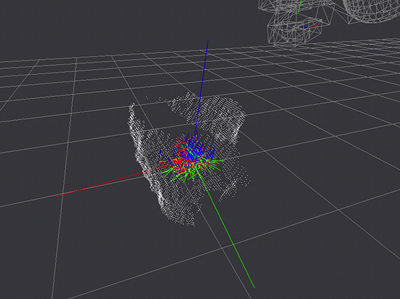
\includegraphics[height=5.0cm,width=.48\columnwidth]{img/from_rss/high_dim_filter}
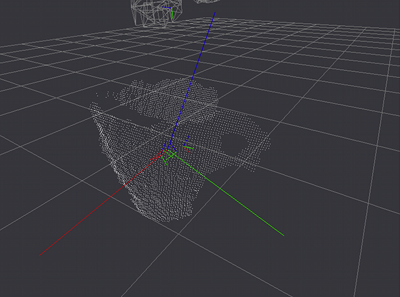
\includegraphics[height=5.0cm,width=.48\columnwidth]{img/from_rss/low_dim_filter}
}
\vspace{0.8mm}
\centerline{
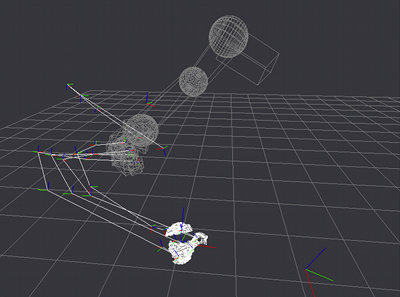
\includegraphics[height=5.0cm,width=.48\columnwidth]{img/from_rss/unoptimised_trajectory}
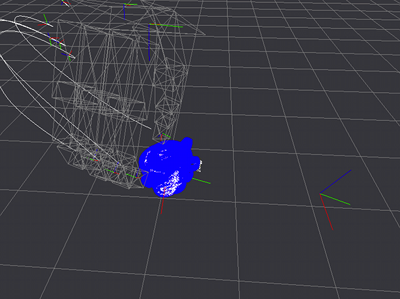
\includegraphics[height=5.0cm,width=.48\columnwidth]{img/from_rss/optimised_trajectory}
}
\caption[IG planner for dexterous grasping]{Top row: The high dimensional belief state used to track object pose (left); the low dimensional filter used for planning (right). Bottom row: The unoptimised PRM plan for fingers and wrist (left); the optimised and smoothed trajectory (right).}
\label{fig:spam.plan.example}
\end{figure}

\subsection{Planning a trajectory to maximise information gain}\label{sec:ch06:heuristic}

The implementation of this planner uses a modified version of Probabilistic Roadmap (PRM),~\citep{bib:kavraki_1996}, to plan trajectories and detect collisions. As discussed in Sec.~\ref{subsec:ch03:multi_query}, the PRM algorithm is composed of two phases: i) \emph{learning phase}, in which a connected graph $\mathbf{G}$ of obstacle-free configurations of the robot is generated and, ii) \emph{query phase}, in which a path is searched for a given pair of configurations $x_{root},x_{goal}$. However the computational cost for the learning phase grows very fast with respect to the dimensionality of the problem. This planner therefore incrementally builds connections between neighbouring nodes during the query phase. 
Given a pair $\langle x_{root}, goal\rangle$ which describes the root state in configuration space, $\mathbb{R}^n$, and goal state in workspace, $SE(3)$, of the trajectory, this planner uses an A* algorithm to find a minimum cost trajectory in obstacle-free joint space according to:
\begin{equation}
c(x) = c_1(x,x_{root}) + c_2(x,x',\hat{x}_{goal})
\end{equation} 
where $x,x'\in\mathbb{R}^n$ and $x'\in Neighbour(x)$, $\hat{x}_{goal}$ is a reachable goal configuration for the robot computed by inverse kinematics, $c_1(x,x_{root})$ is the cost-to-reach $x$ from $x_{root}$ and $c_2(x,x',\hat{x}_{goal})$ is a linear combination of the cost-to-go from $x$ to a neighbour node $x'$ and the expected cost-to-go from $x'$ to the target. I implemented $c_1(\cdot)$ as a cumulative discounted and rewarded travelled distances. More specifically, I define 
%Initially a random graph, $\mathbf{G}$, of robot configurations in obstacle-free space is generated and then a path to a given goal state is searched according to some user defined heuristic. 
%Given a pair $\langle x_{root}, goal\rangle$ which describe the root state in configuration space, $\mathbb{R}^n$, and goal state in workspace, $SE(3)$, of the trajectory, our PRM-based algorithm finds a joint space trajectory as follows:
%\begin{itemize}
%\item adds $x_{root}$ to $\mathbf{G}$
%\item finds a obstacle-free configuration $\hat{x}_{goal}$ which is a reachable goal configuration for the robot
%\item evaluates each node $x$ in the graph $\mathbf{G}$ according to 
%\begin{equation}
%\begin{aligned}
%c_1(x,x_{root},\hat{x}_{goal})=&\alpha d(x,x_{root})\\
%&+\beta d(x,\hat{x}_{goal})+\gamma d_{cfg}(x)
%\end{aligned}
%\end{equation} 
%\item starting from $x_{root}$ finds all its neighbouring nodes within a given threshold and compute the follows cost-to-go function
\begin{equation}\label{eq:cost2}
\begin{aligned}
c_2(x,x',\hat{x}_{goal})=\alpha d_{bound}(x,x') +\beta &d(x',\hat{x}_{goal})\\
&+\gamma d_{cfg}(x)
\end{aligned}
\end{equation} 
%\item finds a path from $x_{root}$ to $\hat{x}_{goal}$ which minimises $c_2(\cdot)$ using A* algorithm
%\end{itemize}
where $\alpha,\beta,\gamma\in\mathbb{R}$, $d(\cdot)$ is a distance function in $SE(3)$ which linearly combine rotational and translational distances in workspace\footnote{For the sake of simplicity, I reduce the mathematical notation by writing $d(x,x')$ instead of d(W(x),W(x')).}. For $d_{bound}(\cdot)$, let $\mathcal{B}_n(r)=\{x\in\mathbb{R}^n|x^Tx\leq r^2\}$ and $\mathcal{B}(r_{l},r_{a})=\{A=[\begin{smallmatrix}R&p\\ 0&1\end{smallmatrix}]\in SE(3)|p^Tp\leq r_{l}^2\text{ and } 1-\langle Q(R),Q(R)\rangle\leq r_{a}^2\}$\footnote{I simplified the notation $\mathcal{B}_{SE(3)}(\cdot)$ in $\mathcal{B}(\cdot)$ for pratical reasons.} denote repectively the $r$-ball in $\mathbb{R}^n$ and in $SE(3)$, then $b_{bound}(x,x')$ is defined as %$\zeta d(x,x')+(1-\zeta)||x-x'||_2$ with $\zeta\in(0,1)$ if $\mathcal{W}(x)-W(x')\in\mathcal{B}_{SE(3)}(r)$ and $x-x'\in\mathcal{B}_n(r')$ or $+\infty$ otherwise.
$$
d_{bound}(x,x')=
\begin{cases}
\psi(x,x')& \text{if }W(x)-W(x')\in\mathcal{B}(r_{l},r_{a}) \\
& \text{and }x-x'\in\mathcal{B}_n(r) \\
+\infty & \text{otherwise}
\end{cases}
$$
where $Q(\cdot)$ is the Quaternion operator for $R\in SO(3)$, $\langle q_1,q_2\rangle$ is the inner product of two quaternions, $r_{l}, r\in\mathbb{R}, r_{a}\in (0,1)$, and $\psi(x,x')=\zeta d(x,x')+(1-\zeta)||x-x'||_2$ with $\zeta\in(0,1)$.
%is an \emph{ad-hoc} distance function that takes into account also distance in the joint space and has the good property of penalising pairs of configurations far away from each others 
Finally, $d_{cfg}(\cdot)$ is a function which penalises dangerous configurations of the robot (i.e. close to joint limits). %Our PRM-based algorithm uses $d_{bound}(\cdot)$ and $d_{cfg}(\cdot)$ to generate edges only between safe robot's configurations (PRM nodes) which are close enough in joint space, and transitions between one configuration and the other can be easily computed by inverse kinematic.

I redefine the heuristic $c_2(\cdot)$ in order to reward informative tactile explorations while attempting to reach the goal state (described as a target configuration of the manipulator). 
%Let $x\in G$ define a obstacle-free configuration of the robot in the PRM, then iteratively the PRM algorithm minimises the following cost function:
% \begin{equation}\label{eq:modifiedcost2}
%\min_{x'\in G}{\alpha \mathcal{J}(x, x', p^{1:k})d_{bound}(x,x')+\beta d_Q(x',\hat{x}_{goal})+\gamma d_{cfg}(x')}
%\end{equation}
%
%Our main contribution is the definition of a new set of heuristics which encode the uncertainty over the object pose. We define,  
%\begin{equation}\label{eq:newcost1}
%\begin{aligned}
%\bar{c}_1(x,x_{root},\hat{x}_{goal},Q)=&\alpha d(x,x_{root})\\
%&+\beta d_Q(x,\hat{x}_{goal})+\gamma d_{cfg}(x)
%\end{aligned}
%\end{equation}
%and 
\begin{equation}\label{eq:newcost2}
\begin{aligned}
\bar{c}_2(x,x',\hat{x}_{goal},A,p^{1:k})=&\alpha \mathcal{J}(x,x',p^{1:k})d_{bound}(x,x')\\
&+\beta d_A(x',\hat{x}_{goal})+\gamma d_{cfg}(x')
\end{aligned}
\end{equation}
where $A$ is the diagonal covariance matrix of the sampled states, for any column vector $a,\mu\in\mathbb{R}^n$, $d_A(a, \mu)=\sqrt{(a-\mu)^TA^{-1}(a-\mu)}$ is the Mahalanobis distance centered in $\mu$ and $\mathcal{J}(x,x',p^{1:k})\in(0,1]$ is a factor which rewards trajectories with a large difference between expected observations if the object is at the expected location, $p^1$, versus observations that would be expected if the object is at other poses, $p^{2:k}$, sampled from the distribution of poses associated with the object's positional uncertainty:
\begin{equation}\label{eq:modifiedcost}
\mathcal{J}(x,x',p^{1:k})=\frac{1}{k-1}\sum_{i=2}^k{e^{-\Phi(x,x',p^i)}}
\end{equation}
where:
$$
\Phi(x,x',p^i)=||h_t(x,x',p^i)-h_t(x,x',p^1)||_2
$$
for each $i\in[2,k]$ and $h_t(x,x',p^i)$ is sequence of probability of reading a contact travelling from state $x$ to $x'$. In this implementation $h_t(x,x',p^i)=h(x',p^i)$. In other words, I evaluate the likelihood of making a contact while moving from state $x$ to $x'$ as the likelihood of making a contact only in the next state $x'$.
Note that this observational model is designed to conserve (\ref{eq:newcost2}) as in (\ref{eq:cost2}) when the likelihood of observing a tactile contact is zero. In fact, for robot configurations in which the distance to the sampled poses is larger than a threshold, $d_{max}$, the cost function $\mathcal{J}(\cdot)$  is equal to 1. However I also encode uncertainty in the second factor of the heuristics, $d_A(\cdot)$, which evaluates the expected distance to the goal configuration. In this way the planner also copes with pose uncertainty at the early stages of the trajectory, when the robot is still too far away from the object to observe any contacts. 

\subsection{Planning for Dexterous manipulator}

In order to compute a dexterous trajectory which allows us to plan movement for both arm and fingers we need to break down the curse of dimensionality or, equivalently, increase the number of sampled configurations to properly cover the configuration space. 

The proposed solution is to build a hierarchical planner. First a PRM is constructed only in the arm configuration space in order to find a global path between the $x_{root},\hat{x}_{goal}$. It is worth noticing that in this phase the rest of the joints of the manipulator are interpolated in order to have a smooth passage from $x_{root}$ to $\hat{x}_{goal}$. Then the planned trajectory is refined by constructing a new PRM in the entire configuration space of the manipulator (e.g. arm + hand joint space) along the global path. In other words, this approach limits the new PRM to explore only the subspace nearby the configurations which compose the global path.  
Subsequently an optimisation procedure is executed along the trajectory to generate a smoother transition from one configuration to the next.

This approach enable us to plan dexterous reach-to-grasp trajectories up to 21 DoF with only 1,000 sampled configurations. Note that this is the same order of magnitude that it is used in practise for planning trajectories of much simpler 6 DoF robot manipulators. 

\subsection{Belief update}

Once a trajectory is executed and a real (unexpected) observation $y$ is detected, the belief state is updated according to the Bayes' rule. The belief state is represented as a set of $N$ particles $b_t=\{b_t^z\}_{z=1}^{N}$. In a particle filter fashion the weight of each particle $b_t^z$, $z\in\{1,\ldots,N\}$ is updated as follows
$$
Pr(y|x, b_t^z)=\prod_{j\in\hat{M}}{Pr(y_{t}(j)|x_{t}(j),b_t^z)}
$$
and then re-sampling is performed to generate a posterior distribution $b_{t+1}$ as new set of particles $\{b_{t+1}^z\}_{z=1}^{N}$.

In simulation this approach assumes that there are no false detections. However it is possible to distinguish whether or not a contact occurs between the object to be grasped and the robot's end-effector. For example, in case a contact with the environment is detected, the algorithm skips the belief update step and moves the robot back to a safe configuration before triggering the re-planning.

